%Problem Set 5
%%%%%%%%%%%%%%%%%%%%%%%%%%%%%%%%%%%%%%%%%%%%%%%%

%I) DEFINE DOCUMENTCLASS AND LOAD ALL REQUIRED PACKAGES

\documentclass[11pt,reqno]{amsart}\usepackage[]{graphicx}\usepackage[]{color}
% maxwidth is the original width if it is less than linewidth
% otherwise use linewidth (to make sure the graphics do not exceed the margin)
\makeatletter
\def\maxwidth{ %
  \ifdim\Gin@nat@width>\linewidth
    \linewidth
  \else
    \Gin@nat@width
  \fi
}
\makeatother

\definecolor{fgcolor}{rgb}{0.196, 0.196, 0.196}
\newcommand{\hlnum}[1]{\textcolor[rgb]{0.063,0.58,0.627}{#1}}%
\newcommand{\hlstr}[1]{\textcolor[rgb]{0.063,0.58,0.627}{#1}}%
\newcommand{\hlcom}[1]{\textcolor[rgb]{0.588,0.588,0.588}{#1}}%
\newcommand{\hlopt}[1]{\textcolor[rgb]{0.196,0.196,0.196}{#1}}%
\newcommand{\hlstd}[1]{\textcolor[rgb]{0.196,0.196,0.196}{#1}}%
\newcommand{\hlkwa}[1]{\textcolor[rgb]{0.231,0.416,0.784}{#1}}%
\newcommand{\hlkwb}[1]{\textcolor[rgb]{0.627,0,0.314}{#1}}%
\newcommand{\hlkwc}[1]{\textcolor[rgb]{0,0.631,0.314}{#1}}%
\newcommand{\hlkwd}[1]{\textcolor[rgb]{0.78,0.227,0.412}{#1}}%
\let\hlipl\hlkwb

\usepackage{framed}
\makeatletter
\newenvironment{kframe}{%
 \def\at@end@of@kframe{}%
 \ifinner\ifhmode%
  \def\at@end@of@kframe{\end{minipage}}%
  \begin{minipage}{\columnwidth}%
 \fi\fi%
 \def\FrameCommand##1{\hskip\@totalleftmargin \hskip-\fboxsep
 \colorbox{shadecolor}{##1}\hskip-\fboxsep
     % There is no \\@totalrightmargin, so:
     \hskip-\linewidth \hskip-\@totalleftmargin \hskip\columnwidth}%
 \MakeFramed {\advance\hsize-\width
   \@totalleftmargin\z@ \linewidth\hsize
   \@setminipage}}%
 {\par\unskip\endMakeFramed%
 \at@end@of@kframe}
\makeatother

\definecolor{shadecolor}{rgb}{.97, .97, .97}
\definecolor{messagecolor}{rgb}{0, 0, 0}
\definecolor{warningcolor}{rgb}{1, 0, 1}
\definecolor{errorcolor}{rgb}{1, 0, 0}
\newenvironment{knitrout}{}{} % an empty environment to be redefined in TeX

\usepackage{alltt}   %keep it simple
\usepackage{hyperref}
\usepackage{graphicx}      % for fancy graphics
\usepackage{setspace}      % for basic formatting
\usepackage{enumerate}     % for more flexibility with numbered lists
%\SweaveOpts{keep.source=TRUE}  %KEY - this preserves R formatting and comments

% You may need to load all or some of these packages -
%follow the instructions on our course web site under "Help with LaTex"

%II) PREAMBLE
%%%%%%%%%%%%%%%%%%%%%%%%%%%%%%%%%%%%%%%%%%%%%%%%%%
\pagestyle{plain} %puts page number center bottom
\setlength{\topmargin}{0in}
\setlength{\textheight}{8.5in}
\setlength{\oddsidemargin}{.0in}
\setlength{\evensidemargin}{.0in}
\setlength{\textwidth}{6.5in}
\setlength{\footskip}{.5in}
\setlength{\parindent}{0in} %suppress indentation
%\onehalfspacing

\newcommand{\mlt}[1]{\mathbf{#1}} %matrix bold for Latin symbols
\newcommand{\mgr}[1]{\mathbf{#1}}%matrix bold for Greek symbols
\newcommand{\kR}{\tt R\rm{} }%shortcut for "R" symbol
\newcommand{\ksp}{\vspace{0.1in}}   % insert some space between chunks
%feel free to add your own shortcuts  - here a mine:
\newcommand{\kl}{\left(}
\newcommand{\kr}{\right)}
\newcommand{\kll}{\left\{}
\newcommand{\krr}{\right\}}
\newcommand{\kmu}{\mgr{\mu}}
\newcommand{\kpsi}{\mgr{\psi}}
\newcommand{\kphi}{\mgr{\phi}}
\newcommand{\kgam}{\mgr{\gamma}}
\newcommand{\ktheta}{\mgr{\theta}}
\newcommand{\kbeta}{\mgr{\beta}}
\newcommand{\kdelta}{\mgr{\delta}}
\newcommand{\kt}{^{\prime}}
\newcommand{\kdel}{\partial}
\newcommand{\kdot}{\kl . \kr}
\newcommand{\keps}{\epsilon}
\newcommand{\kx}{\mlt{x}}
\newcommand{\kX}{\mlt{X}}
\newcommand{\kV}{\mlt{V}}
\newcommand{\kM}{\mlt{M}}
\newcommand{\kP}{\mlt{P}}
\newcommand{\ky}{\mlt{y}}
\newcommand{\kb}{\mlt{b}}
\newcommand{\kc}{\mlt{c}}
\newcommand{\ki}{\mlt{i}}
\newcommand{\ke}{\mlt{e}}
\newcommand{\klam}{\lambda}
\newcommand{\kp}{\mlt{p}}
\newcommand{\kprob}{\text{prob}}
\newcommand{\kz}{\mlt{z}}
\newcommand{\ksig}{\sigma^2}
\newcommand{\kSig}{\mgr{\Sigma}}
\newcommand{\klog}{\text{log}}
\newcommand{\kols}{\kl \kX\kt\kX\kr^{-1}\kX\kt\ky}
\newcommand{\kSSE}{\kl \ky-\kX\kb\kr\kt\kl\ky-\kX\kb\kr}

\newenvironment{nouppercase}{%
  \let\uppercase\relax%
  \renewcommand{\uppercasenonmath}[1]{}}{}
  
%%%%%%%%%%%%%%%%%%%%%%%%
\IfFileExists{upquote.sty}{\usepackage{upquote}}{}
\begin{document}
%\SweaveOpts{concordance=TRUE}
%%%%%%%%%%%%%%%%%%%%%%%%

%III) TOP MATTER INFORMATION
\title{Problem Set 5}
\author{Nima Mohammadi \\ \href{mailto:nimamo@vt.edu}{\textbf{nimamo@vt.edu}}} %ENTER YOUR NAME HERE
\begin{nouppercase}
\maketitle %this comes at the end of the top matter to set it.
\end{nouppercase}








%%%%%%%%%%%%%%%%%%%%%%%%%%%%%%%%%%%%%%%%%%%%%%%%%%%%%%%%%%%%%%%%%%%%%%%%
\section{Q1: Serial correlation}
%%%%%%%%%%%%%%%%%%%%%%%%%%%%%%%%%%%%%%%%%%%%%%%%%%%%%%%%%%%%%%%%%%%%%%%%
(See scripts \texttt{mod4s3a} and  \texttt{mod4s3b} for guidance) 
Consider Greene's gasoline consumption data (on the web under "gasoline" in tab-delimited .txt  format).  The variables are as follows:
\vspace{0.1in}

\begin{footnotesize}
\begin{enumerate}
\item  Year = Year, 1953-2004, 
\item   GasExp = Total U.S. gasoline expenditure, in thousands
\item   Pop = U.S. total population in thousands 
\item   GasP = Price index for gasoline, 
\item   Income = Per capita disposable income, 
\item   Pnc = Price index for new cars, 
\item   Puc = Price index for used cars, 
\item  Ppt = Price index for public transportation, 
\item   Pd = Aggregate price index for consumer durables, 
\item  Pn = Aggregate price index for consumer nondurables, 
\item  Ps = Aggregate price index for consumer services. 
\end{enumerate}
\end{footnotesize}
\vspace{0.1in}

The textbook analyzes a model using these data in the context of autocorrelation on pp. 649-650.

Load the data into R, and specify Greene's model on p. 649 (6th edition), p. 927 (7th edition). Your dependent variable should be log[(GasExp)/(Pop*GasP)]. Your regressors should be:

\vspace{0.1in}
\begin{footnotesize}
\begin{enumerate}
\item   constant 
\item   income = log(Per capita disposable income)
\item  GasP = log(Price index for gasoline)
\item   Pnc = log(Price index for new cars) 
\item   Puc = log(Price index for used cars) 
\item   time index
\end{enumerate}
\end{footnotesize}
\vspace{0.1in}

\begin{knitrout}
\definecolor{shadecolor}{rgb}{1, 1, 1}\color{fgcolor}\begin{kframe}
\begin{alltt}
\hlstd{data} \hlkwb{<-} \hlkwd{read.table}\hlstd{(}\hlstr{'/Users/nima/AAEC5126/data/gasoline.txt'}\hlstd{,} \hlkwc{sep}\hlstd{=}\hlstr{"\textbackslash{}t"}\hlstd{,} \hlkwc{header}\hlstd{=}\hlnum{FALSE}\hlstd{)}

\hlkwd{colnames}\hlstd{(data)} \hlkwb{<-} \hlkwd{c}\hlstd{(}\hlstr{"Year"}\hlstd{,} \hlstr{"GasExp"}\hlstd{,} \hlstr{"Pop"}\hlstd{,} \hlstr{"GasP"}\hlstd{,}\hlstr{"Income"}\hlstd{,} \hlstr{"Pnc"}\hlstd{,} \hlstr{"Puc"}\hlstd{,}
                    \hlstr{"Ppt"}\hlstd{,} \hlstr{"Pd"}\hlstd{,} \hlstr{"Pn"}\hlstd{,} \hlstr{"Ps"}\hlstd{)}
\hlkwd{attach}\hlstd{(data)}
\end{alltt}
\end{kframe}
\end{knitrout}

To create the last regressor (time index), you need to translate the year - variable into a running index from 1:52. Label this variable "$t_i$". 

\begin{knitrout}
\definecolor{shadecolor}{rgb}{1, 1, 1}\color{fgcolor}\begin{kframe}
\begin{alltt}
\hlstd{y} \hlkwb{<-} \hlkwd{log}\hlstd{(GasExp} \hlopt{/} \hlstd{(Pop} \hlopt{*} \hlstd{GasP))}

\hlstd{Income} \hlkwb{<-} \hlkwd{log}\hlstd{(Income)}
\hlstd{GasP} \hlkwb{<-} \hlkwd{log}\hlstd{(GasP)}
\hlstd{Pnc} \hlkwb{<-} \hlkwd{log}\hlstd{(Pnc)}
\hlstd{Puc} \hlkwb{<-} \hlkwd{log}\hlstd{(Puc)}
\hlstd{t_i} \hlkwb{<-} \hlstd{data}\hlopt{$}\hlstd{Year} \hlopt{-} \hlkwd{min}\hlstd{(data}\hlopt{$}\hlstd{Year)} \hlopt{+} \hlnum{1}
\end{alltt}
\end{kframe}
\end{knitrout}

\begin{enumerate}
\item 
Run a simple OLS model.  (Note: Greene's results on p. 650 / 927 are a bit off, but close).  Comment on the significance levels of each regressor (ignore the constant term).  Are the signs of significant regressors as expected? Explain.\\

\begin{knitrout}
\definecolor{shadecolor}{rgb}{1, 1, 1}\color{fgcolor}\begin{kframe}
\begin{alltt}
\hlstd{X} \hlkwb{<-} \hlkwd{cbind}\hlstd{(}\hlkwd{rep}\hlstd{(}\hlnum{1}\hlstd{,} \hlkwd{nrow}\hlstd{(data)), Income, GasP, Pnc, Puc, t_i)}
\hlstd{k} \hlkwb{<-} \hlkwd{ncol}\hlstd{(X)}
\hlstd{n} \hlkwb{<-} \hlkwd{nrow}\hlstd{(X)}

\hlcom{#OLS estimator}
\hlstd{bols} \hlkwb{<-} \hlkwd{solve}\hlstd{((}\hlkwd{t}\hlstd{(X))} \hlopt \hlstd{X)} \hlopt \hlstd{(}\hlkwd{t}\hlstd{(X)} \hlopt \hlstd{y)}
\hlstd{e} \hlkwb{<-} \hlstd{y} \hlopt{-} \hlstd{X} \hlopt \hlstd{bols} \hlcom{# residuals}
\hlstd{SSR} \hlkwb{<-} \hlstd{(}\hlkwd{t}\hlstd{(e)} \hlopt \hlstd{e)}\hlcom{#sum of squared residuals}
\hlstd{s2} \hlkwb{<-} \hlstd{(}\hlkwd{t}\hlstd{(e)} \hlopt \hlstd{e)} \hlopt{/} \hlstd{(n} \hlopt{-} \hlstd{k)} \hlcom{#estimated variance of "eps"}
\hlstd{s2ols} \hlkwb{<-} \hlstd{s2} \hlcom{#for Hausman test below}
\hlstd{Vb} \hlkwb{<-} \hlstd{s2[}\hlnum{1}\hlstd{,} \hlnum{1}\hlstd{]} \hlopt{*} \hlkwd{solve}\hlstd{((}\hlkwd{t}\hlstd{(X))} \hlopt \hlstd{X)} \hlcom{# estimated VCOV matrix of bols}
\hlstd{se} \hlkwb{=} \hlkwd{sqrt}\hlstd{(}\hlkwd{diag}\hlstd{(Vb))} \hlcom{# get the standard erros for your coefficients}
\hlstd{tval} \hlkwb{=} \hlstd{bols} \hlopt{/} \hlstd{se} \hlcom{# get your t-values}
\end{alltt}
\end{kframe}
\end{knitrout}

\ksp
% latex table generated in R 3.6.2 by xtable 1.8-4 package
% Fri May  1 14:59:42 2020
\begin{table}[ht]
\centering
\caption{OLS output} 
\begin{tabular}{lrrr}
  \hline
variable & estimate & s.e. & t \\ 
  \hline
constant & -26.6753 & 2.0005 & -13.3340 \\ 
  log(income) & 1.6246 & 0.1952 & 8.3227 \\ 
  log(GasP) & -0.0539 & 0.0422 & -1.2782 \\ 
  log(Pnc) & -0.0834 & 0.1766 & -0.4725 \\ 
  log(Puc) & -0.0847 & 0.1024 & -0.8272 \\ 
  t\_i & -0.0139 & 0.0048 & -2.9149 \\ 
   \hline
\end{tabular}
\end{table}


The results show that the coefficients of log(income) and time are significant at 1\% and 5\% levels. The sign of the coefficient of the variable "log of Per capita disposable income" is positive which means that a 1\% increase in Per capita disposable income leads to 1.625\% increase in [(GasExp)/(Pop*GasP)]. Subsequently, whenever per capita disposable income increases people may travel more because they will make more use of their cars and this would lead to an increase of gasoline expenditure.  Therefore the sign of significant regressor "income" is expected. Going ahead in time has different impacts on gas consumption. First, along time technology improves and cars use less gas for the same milage, this suggests negative coefficient. Second, overtime individuals are become wealthier, as percapita income increases, more people can afford cars and this increases the gas usage and suggest positive effect. Therefore, the true sign for time coefficient depends on which effect is larger. However, the results show negative impact of time.  \\

\item
Generate OLS residuals (call them "$\ke$") and plot them against time (year).  The pattern should look a lot like the graph on p. 650 / 928.  Does it indicate autocorrelation - why or why not? If so, is it suggestive of positive or negative autocorrelation - explain. \\ 

\begin{figure}[!ht]
\centering
\begin{knitrout}
\definecolor{shadecolor}{rgb}{1, 1, 1}\color{fgcolor}
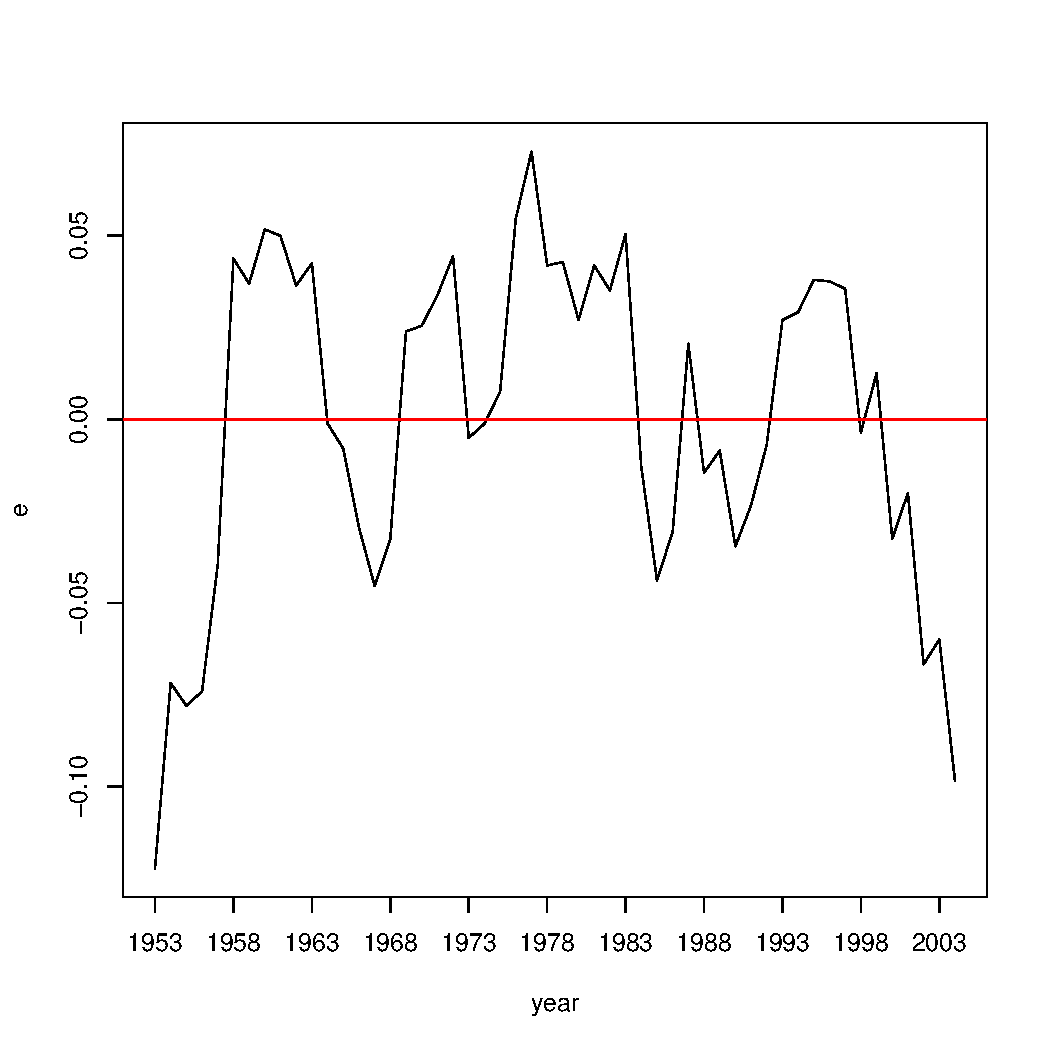
\includegraphics[width=\maxwidth]{figure/theme-R5-1} 

\end{knitrout}
\caption{OLS residual plots}
\label{fig:scatter1}
\end{figure}

The figure shows that the existence of consecutive upward and downward movements in residuals. We know that this plot suggests positive autocorrelation. That is for positive correlation, positive (negative) residuals tend to be followed by positive (negative) residuals. \\


\item
Perform a Breusch-Godfrey multiplier test for AR(1).  State the null and alternative hypotheses, the computed p-value and your decision regarding the null (at 5\% level of significance).\\

\begin{kframe}
\begin{alltt}
\hlstd{elag} \hlkwb{<-} \hlstd{e[}\hlnum{1}\hlopt{:}\hlstd{(n} \hlopt{-} \hlnum{1}\hlstd{)]}

\hlstd{e0lag} \hlkwb{<-} \hlkwd{c}\hlstd{(}\hlnum{0}\hlstd{, elag)} \hlcom{# fill first position with 0 */}
\hlstd{Xo} \hlkwb{=} \hlkwd{cbind}\hlstd{(X, e0lag)} \hlcom{#augment X with a column of lagged residuals}

\hlstd{LM} \hlkwb{<-} \hlstd{n} \hlopt{*} \hlstd{((}\hlkwd{t}\hlstd{(e)} \hlopt \hlstd{Xo} \hlopt \hlkwd{solve}\hlstd{(}\hlkwd{t}\hlstd{(Xo)} \hlopt \hlstd{Xo)}
            \hlopt \hlkwd{t}\hlstd{(Xo)} \hlopt \hlstd{e)} \hlopt{/} \hlstd{(}\hlkwd{t}\hlstd{(e)} \hlopt \hlstd{e))}
\hlstd{pval} \hlkwb{=} \hlnum{1} \hlopt{-} \hlkwd{pchisq}\hlstd{(LM,} \hlnum{1}\hlstd{)}
\end{alltt}
\end{kframe}
\ksp
The Breusch-Godfrey test can be used for a set of alternative hypotheses. Each of which describes a different AR(P) process. Here, our test for P=1 we investigate for process of order 1. That is the null hypothesis will be:
\ksp
\begin{itemize}
\item $H_0:$ No autocorrelation of order P=1
\item $H_a:$ Autoregressive or Moving average of order P=1
\end{itemize}

\ksp
The test statistic for this test is

$$\mathrm{BG}=T\left(\frac{\varepsilon^{\prime} \mathbf{X}_{0}\left(\mathbf{X}_{0}^{\prime} \mathbf{X}_{0}\right)^{-1} \mathbf{X}_{0}^{\prime} \varepsilon}{\varepsilon^{\prime} \varepsilon}\right) \sim \chi^{2}(P)$$

The BG-statistic for this test is 27.182.\\*
The degrees of freedom for the test are 1.\\*
The corresponding p-value is 0.\\* 
So the null hypothesis will be rejected, which is "there is no autocorrelation" at 5\%  and 1\% level of significance. We cannot say there is no autocorrelation.\\
\ksp

\item
Compute the Durbin-Watson statistic.  State the null and alternative hypotheses, the appropriate degrees of freedom, the appropriate critical values from the DW Table at $\alpha=0.05$ (textbook or google on the web), and your decision regarding the null. (the DW value should be the same as the one mentioned in Greene, up two the first 2 decimals).\\

\begin{kframe}
\begin{alltt}
\hlstd{ecurr} \hlkwb{<-} \hlstd{e[}\hlnum{2}\hlopt{:}\hlstd{n]}
\hlstd{elag} \hlkwb{<-} \hlstd{e[}\hlnum{1}\hlopt{:}\hlstd{(n} \hlopt{-} \hlnum{1}\hlstd{)]}
\hlstd{d} \hlkwb{<-} \hlstd{(}\hlkwd{t}\hlstd{(ecurr} \hlopt{-} \hlstd{elag)} \hlopt \hlstd{(ecurr} \hlopt{-} \hlstd{elag))} \hlopt{/} \hlstd{(}\hlkwd{t}\hlstd{(e)} \hlopt \hlstd{e)}
\end{alltt}
\end{kframe}
\ksp

The test statistic is

$$d=\frac{\left(\varepsilon_{t}-\varepsilon_{t-1}\right)^{\prime}\left(\varepsilon_{t}-\varepsilon_{t-1}\right)}{\varepsilon_{t}^{\prime} \varepsilon_{t}} \approx 2(1-\hat{\rho})$$

\begin{itemize}
\item $\varepsilon_{t}$ = vector of original residuals from OLS\\
\item $\varepsilon_{t-1}$ = vector of lagged residuals\\
\item $\hat{\rho}$ = estimated autocorrelation coefficient from a regression of $\varepsilon_{t}$ on $\varepsilon_{t-1}$\\
\end{itemize}
\ksp
The null and Alternative hypothesis: 

\begin{itemize}
\item $H_0:$ $\rho = 0$ absence of serial correlation\\
\item $H_a:$ $\rho > 0$ positive auotocorrelation\\
\item $H_a:$ $\rho < 0$ negative auotocorrelation\\
\end{itemize}

The decision rule using dL, dU:
\begin{itemize}
\item For $H_a:$ $\rho > 0$: $H_0$ is rejected if d$<$dL; $H_0$ is not rejected if d$>$dU. Inconclusive if dL$<$d$<$dU.

\item For $H_a:$ $\rho < 0$: $H_0$ is rejected if d$>$(4-dL); $H_0$ is not rejected if d$<$(4-dU). Inconclusive if (4-dU)$<$d<(4-dL)\\
\end{itemize}

For this specific case our null and alternative hypothesis is:
\begin{itemize}
\item $H_0:$ $\rho = 0$\\
\item $H_a:$ $\rho > 0$\\
\end{itemize}

The DW-statistic for this test is 0.424.
The sample size is 52.
The column space of X is 6.\\

According to the Durbin-Watson table, the lower bound of d (dL) is 1.34. So d=.424 < dL= 1.34. Thus, we reject the null hypothesis. So, we have positive autocorrelation.\\

\ksp
\ksp

\item
Estimate robust OLS with  Newey-West corrected standard errors. (In $\kR$, you can use 
\begin{verbatim} L<-ceiling(n^(1/4)) \end{verbatim} for the lag indicator, where n is the sample size).\\

\begin{kframe}
\begin{alltt}
\hlstd{L} \hlkwb{<-} \hlkwd{ceiling}\hlstd{(n} \hlopt{^} \hlstd{(}\hlnum{1} \hlopt{/} \hlnum{4}\hlstd{))}
\hlcom{# rounds upwards to nearest integer;}
\hlcom{# this would be the generic choice}
\hlstd{H} \hlkwb{<-} \hlkwd{matrix}\hlstd{(}\hlnum{0}\hlstd{, k, k)}

\hlkwa{for} \hlstd{(j} \hlkwa{in} \hlnum{1}\hlopt{:}\hlstd{L) \{}
  \hlstd{t} \hlkwb{<-} \hlstd{j} \hlopt{+} \hlnum{1}
  \hlstd{G} \hlkwb{<-} \hlkwd{matrix}\hlstd{(}\hlnum{0}\hlstd{, k, k)}
  \hlkwa{for} \hlstd{(i} \hlkwa{in} \hlstd{t}\hlopt{:}\hlstd{n)  \{}
    \hlstd{m} \hlkwb{<-} \hlstd{(}\hlnum{1} \hlopt{-} \hlstd{(j} \hlopt{/} \hlstd{(L} \hlopt{+} \hlnum{1}\hlstd{)))} \hlopt{*} \hlstd{e[i]} \hlopt{*} \hlstd{e[i} \hlopt{-} \hlstd{j]} \hlopt{*}
      \hlstd{(}\hlkwd{t}\hlstd{(X[i, ,} \hlkwc{drop} \hlstd{=} \hlnum{FALSE}\hlstd{])} \hlopt \hlstd{X[i} \hlopt{-} \hlstd{j, ]} \hlopt{+} \hlkwd{t}\hlstd{(X[i} \hlopt{-} \hlstd{j, ,} \hlkwc{drop} \hlstd{=} \hlnum{FALSE}\hlstd{])} \hlopt \hlstd{X[i, ])}
    \hlcom{#drop=FALSE forces the transpose to be a column vector}
    \hlstd{G} \hlkwb{<-} \hlstd{G} \hlopt{+} \hlstd{m}
  \hlstd{\}}
  \hlstd{H} \hlkwb{<-} \hlstd{H} \hlopt{+} \hlstd{G}
\hlstd{\}}
\hlstd{e} \hlkwb{<-} \hlkwd{as.vector}\hlstd{(e)}
\hlstd{S1} \hlkwb{<-} \hlstd{(}\hlkwd{t}\hlstd{(X)} \hlopt \hlkwd{diag}\hlstd{(e} \hlopt{^} \hlnum{2}\hlstd{)} \hlopt \hlstd{X)} \hlopt{+} \hlstd{H}
\hlstd{Vb} \hlkwb{<-} \hlkwd{solve}\hlstd{((}\hlkwd{t}\hlstd{(X))} \hlopt \hlstd{X)} \hlopt \hlstd{S1} \hlopt \hlkwd{solve}\hlstd{((}\hlkwd{t}\hlstd{(X))} \hlopt \hlstd{X)}
\hlstd{se} \hlkwb{=} \hlkwd{sqrt}\hlstd{(}\hlkwd{diag}\hlstd{(Vb))}
\hlstd{tval} \hlkwb{=} \hlstd{bols} \hlopt{/} \hlstd{se}
\end{alltt}
\end{kframe}

\ksp
% latex table generated in R 3.6.2 by xtable 1.8-4 package
% Fri May  1 14:59:42 2020
\begin{table}[ht]
\centering
\caption{Robust OLS output} 
\begin{tabular}{lrrr}
  \hline
variable & estimate & s.e. & t \\ 
  \hline
constant & -26.675 & 2.408 & -11.079 \\ 
  log(income) & 1.625 & 0.243 & 6.676 \\ 
  log(gasP) & -0.054 & 0.054 & -1.003 \\ 
  log(pnc) & -0.083 & 0.164 & -0.509 \\ 
  log(puc) & -0.085 & 0.104 & -0.818 \\ 
  t\_i & -0.014 & 0.007 & -1.978 \\ 
   \hline
\end{tabular}
\end{table}

\ksp

\item
Compute the Prais-Winsten FGLS estimator.  (The results will be a bit different than those given in Greene - he uses a slightly different estimation approach).\\

\begin{kframe}
\begin{alltt}
\hlcom{# Step 1: Get a consistent estimate of rho:}
\hlstd{rho} \hlkwb{<-}
  \hlkwd{solve}\hlstd{(}\hlkwd{t}\hlstd{(elag)} \hlopt \hlstd{elag)} \hlopt \hlkwd{t}\hlstd{(elag)} \hlopt \hlstd{ecurr} \hlcom{#OLS solution for our}
\hlcom{# "e vs. e-lag 1 regression model above}
\hlcom{#}
\hlcom{#Step 2: compose the correlation matrix R}
\hlstd{R} \hlkwb{<-} \hlkwd{matrix}\hlstd{(}\hlnum{0}\hlstd{, n, n)}
\hlstd{up} \hlkwb{<-} \hlkwd{seq}\hlstd{(}\hlnum{1}\hlstd{, (n} \hlopt{-} \hlnum{1}\hlstd{),} \hlnum{1}\hlstd{)}
\hlstd{down} \hlkwb{<-} \hlkwd{seq}\hlstd{((n} \hlopt{-} \hlnum{1}\hlstd{),} \hlnum{1}\hlstd{,}\hlopt{-}\hlnum{1}\hlstd{)}
\hlstd{int} \hlkwb{<-} \hlkwd{c}\hlstd{(rho} \hlopt{^} \hlstd{(down),} \hlnum{1}\hlstd{, rho} \hlopt{^} \hlstd{(up))} \hlcom{#1 by 2*(n-1)+1}
\end{alltt}


{\ttfamily\noindent\color{warningcolor}{\#\# Warning in rho\textasciicircum{}(down): Recycling array of length 1 in array-vector arithmetic is deprecated.\\\#\#\ \  Use c() or as.vector() instead.}}

{\ttfamily\noindent\color{warningcolor}{\#\# Warning in rho\textasciicircum{}(up): Recycling array of length 1 in array-vector arithmetic is deprecated.\\\#\#\ \  Use c() or as.vector() instead.}}\begin{alltt}
\hlkwa{for} \hlstd{(i} \hlkwa{in} \hlnum{1}\hlopt{:}\hlstd{n) \{}
  \hlstd{R[i, ]} \hlkwb{<-} \hlstd{int[(n} \hlopt{-} \hlstd{(i} \hlopt{-} \hlnum{1}\hlstd{))}\hlopt{:}\hlstd{(}\hlkwd{length}\hlstd{(int)} \hlopt{-} \hlstd{(i} \hlopt{-} \hlnum{1}\hlstd{))]}
\hlstd{\}}
\hlcom{#}
\hlcom{#Step 3: compute FGLS estimator}
\hlstd{bgls} \hlkwb{<-} \hlkwd{solve}\hlstd{((}\hlkwd{t}\hlstd{(X))} \hlopt \hlkwd{solve}\hlstd{(R)} \hlopt \hlstd{X)} \hlopt \hlstd{(}\hlkwd{t}\hlstd{(X)} \hlopt \hlkwd{solve}\hlstd{(R)} \hlopt \hlstd{y)}
\hlcom{#}
\hlcom{#Step 4: compute a consistent estimate of sig(eps)}
\hlstd{e} \hlkwb{<-} \hlstd{y} \hlopt{-} \hlstd{X} \hlopt \hlstd{bgls}
\hlstd{sige} \hlkwb{<-} \hlstd{(}\hlnum{1} \hlopt{/} \hlstd{n)} \hlopt{*} \hlkwd{t}\hlstd{(e)} \hlopt \hlkwd{solve}\hlstd{(R)} \hlopt \hlstd{(e)}
\hlcom{#}
\hlcom{#Step 5: Compute consistent variance-covariance matrix for b_fgls}
\hlstd{Om} \hlkwb{<-} \hlstd{sige[}\hlnum{1}\hlstd{,} \hlnum{1}\hlstd{]} \hlopt{*} \hlstd{R}
\hlstd{Vb} \hlkwb{<-} \hlkwd{solve}\hlstd{((}\hlkwd{t}\hlstd{(X))} \hlopt \hlkwd{solve}\hlstd{(Om)} \hlopt \hlstd{X)}
\hlstd{se} \hlkwb{=} \hlkwd{sqrt}\hlstd{(}\hlkwd{diag}\hlstd{(Vb))}
\hlstd{tval} \hlkwb{=} \hlstd{bgls} \hlopt{/} \hlstd{se}
\end{alltt}
\end{kframe}
% latex table generated in R 3.6.2 by xtable 1.8-4 package
% Fri May  1 14:59:42 2020
\begin{table}[ht]
\centering
\caption{FGLS output} 
\begin{tabular}{lrrr}
  \hline
variable & estimate & s.e. & t \\ 
  \hline
constant & -19.557 & 1.746 & -11.203 \\ 
  log(income) & 0.855 & 0.174 & 4.910 \\ 
  log(gasP) & -0.103 & 0.037 & -2.811 \\ 
  log(pnc) & -0.147 & 0.150 & -0.981 \\ 
  log(puc) & -0.013 & 0.073 & -0.175 \\ 
  t\_i & 0.004 & 0.005 & 0.869 \\ 
   \hline
\end{tabular}
\end{table}



\item
Compare your original OLS estimates, the robust estimates, and the FGLS results and elaborate: \\
    \begin{enumerate}
      \item 	Compare the s.e.'s and t-values between OLS and robust OLS. Are there any noteworthy changes in significance levels? 
      \ksp
      
      The estimates for the OLS and the Robust OLS are almost identical. The standard error for the Robust OLS has slightly increased for all the variables except "pnc". Thus all the t values are smaller (in absolute term) in Robust OLS except "pnc". In both of OLS and Robust OLS "log(income)" and "constant'  are significant at 1\%  and 5\% level. But, "log(gasP)", "log(Pnc)" and "log(Puc)" are insignificant in both. So there is no noteworthy changes in significance levels.\\
The time coefficient is different. OLS result suggests that time is significant in both 1\% and 5\% level, but Robust OLS indicates it is not.

\ksp

      \item	Compare the s.e.'s and t-values between the robust OLS and the FGLS model. Are there any noteworthy changes in significance levels?  
      \ksp
      
      The standard errors are smaller in FGLS for all variables. As tables show, "constant" and "log(income)" are significant in  both methods but "log(Pnc)" nad "log(Puc)" are insignificant in both. The difference is in "log(gasP)". Although, it is significant in FGLS at both 1\% and 5\%, it is not significant in Robust OLS at both levels.
      
      \ksp
      
      \item	Assume the main focus of your research is on the effect of "gas prices" on "gas consumption". Overall, which model would you choose? 
      \ksp
      
      Since the error term follows AR(1) process, the structure of R matrix and so $E({\varepsilon\varepsilon\kt})$ are known. Therefore, GLS results are the most efficient and we perefer to choose FGSL model.
      
    \end{enumerate}
\end{enumerate}


\clearpage
\newpage
%%%%%%%%%%%%%%%%%%%%%%%%%%%%%%%%%%%%%%%%%%%%%%%%%%%%%%%%%%%%%%%%%%%%%%%%
\section{Q2: Estimation of treatment effects via regression}
%%%%%%%%%%%%%%%%%%%%%%%%%%%%%%%%%%%%%%%%%%%%%%%%%%%%%%%%%%%%%%%%%%%%%%%%
This question uses home sales data from Connecticut (CT) for 1991-1999. All properties are single-family residential homes located within 0.25 miles of the coastline. The total sample size is 6,327. Of these, 2,439 are located in a spezial flood hazard area (SFHA), which means they have been declared to be at higher risk of flooding than the remaining 3,888 properties outside the SFHA. However, these homes are alse enjoying overall nicer amenities, such as proximity to beach, water, and views. Thus, it is ex-ante not clear which effect will dominate - the flood risk effect or the amenity effect.\\

The outcome variable of interest is sale price, in \$1,000. The main objective of this exercise is to estimate the combined SFHA \& amenity effect on home prices, and check which effect is stronger.\\

The data are sorted by treatment (SFHA=1 properties first, followed by SFHA=0 properties), and by sales date within treatment. The variables are as follows:\\

\begin{enumerate}
\item DQid            original property ID
\item saleyr          year of sale
\item salemonth       month of sale
\item saleday         calendar day of sale
\item saledateE       sale date in elapsed days since 1/1/1960
\item price000        sale price in 1000's of 2014 dollars
\item SFHA            1= located in SFHA zone
\item age             age of structure, years
\item sqft00          square footage, in 100's
\item lot000          lot size, in 1000 sqft
\item bedrooms        total number of bedrooms
\item bathrooms       total number of baths
\item elev10          elevation in meters at 10 meter resolution
\item ISMi            distance to nearest Interstate, miles
\item PAMi            distance to nearest principal artery, miles
\item beaMi           distance to nearest beach, miles
\item hidMi           distance to nearest high-density development, miles
\item coaestMi        miles to nearest coast or estuary                
\item reslkMi         miles to nearest lake, pond, or reservoir
\item ag10            acreage of ag land w/in 1000m, most current
\item ind10           acreage of ind. land w/in 1000m, most current
\item op10            acreage of open land w/in 1000m, most current
\end{enumerate}


The following loads in the data (including all variable names), and saves it immediately in R's internal (``rda'') format:

\ksp
\begin{knitrout}
\definecolor{shadecolor}{rgb}{1, 1, 1}\color{fgcolor}\begin{kframe}
\begin{alltt}
\hlkwd{rm}\hlstd{(}\hlkwc{list}\hlstd{=}\hlkwd{ls}\hlstd{())}
\hlstd{data} \hlkwb{<-} \hlkwd{read.table}\hlstd{(}\hlstr{'/Users/nima/AAEC5126/data/CTfloodzones.txt'}\hlstd{,}
                   \hlkwc{sep} \hlstd{=} \hlstr{"\textbackslash{}t"}\hlstd{,} \hlkwc{header} \hlstd{=} \hlnum{TRUE}\hlstd{)}
\end{alltt}
\end{kframe}
\end{knitrout}
\ksp

\begin{enumerate}
\item 
Let the dependent variable be ``price000,'' the treatment variable ``SFHA,'', and let the explanatory data $\kX$ include all variables listed above from ``age'' to ``op10'' (15 variables), in addition to a constant term where needed.\\

Check for overlap and show results in a table - which explanatory variables raise red flags by exceeding the recommended overlap core of 0.25 (in absolute terms)? Explain in words which group, treated or controls, has relatively larger or smaller values for these red flag variables.\\

\begin{kframe}
\begin{alltt}
\hlkwd{attach}\hlstd{(data)}
\hlstd{n} \hlkwb{<-} \hlkwd{nrow}\hlstd{(data)}
\hlstd{n1} \hlkwb{<-} \hlkwd{sum}\hlstd{(SFHA} \hlopt{==} \hlnum{1}\hlstd{)}
\hlstd{n0} \hlkwb{<-} \hlstd{n} \hlopt{-} \hlstd{n1}
\hlstd{y} \hlkwb{<-} \hlstd{price000}
\hlstd{X} \hlkwb{<-} \hlstd{data[,} \hlnum{8}\hlopt{:}\hlnum{22}\hlstd{]}
\hlcom{#}
\hlstd{y1} \hlkwb{<-} \hlstd{y[}\hlnum{1}\hlopt{:}\hlstd{n1]}
\hlstd{y0} \hlkwb{<-} \hlstd{y[(n1} \hlopt{+} \hlnum{1}\hlstd{)}\hlopt{:}\hlstd{n]}
\hlstd{my1} \hlkwb{<-} \hlkwd{mean}\hlstd{(y1)}
\hlstd{my0} \hlkwb{<-} \hlkwd{mean}\hlstd{(y0)}
\hlstd{sy1} \hlkwb{<-} \hlkwd{sd}\hlstd{(y1)}
\hlstd{sy0} \hlkwb{<-} \hlkwd{sd}\hlstd{(y0)}
\hlstd{ndiffy} \hlkwb{<-} \hlstd{(my1} \hlopt{-} \hlstd{my0)} \hlopt{/} \hlkwd{sqrt}\hlstd{(sy1} \hlopt{^} \hlnum{2} \hlopt{+} \hlstd{sy0} \hlopt{^} \hlnum{2}\hlstd{)}
\hlcom{#}
\hlstd{X1} \hlkwb{<-} \hlstd{X[}\hlnum{1}\hlopt{:}\hlstd{n1, ]}
\hlstd{X0} \hlkwb{<-} \hlstd{X[(n1} \hlopt{+} \hlnum{1}\hlstd{)}\hlopt{:}\hlstd{n, ]}
\hlstd{mX1} \hlkwb{<-} \hlkwd{colMeans}\hlstd{(X1)}
\hlstd{mX0} \hlkwb{<-} \hlkwd{colMeans}\hlstd{(X0)}
\hlstd{sX1} \hlkwb{<-} \hlkwd{apply}\hlstd{(X1,} \hlnum{2}\hlstd{, sd)}
\hlstd{sX0} \hlkwb{<-} \hlkwd{apply}\hlstd{(X0,} \hlnum{2}\hlstd{, sd)}
\hlstd{ndiffX} \hlkwb{<-} \hlkwd{as.vector}\hlstd{((mX1} \hlopt{-} \hlstd{mX0)} \hlopt{/} \hlkwd{sqrt}\hlstd{(sX1} \hlopt{^} \hlnum{2} \hlopt{+} \hlstd{sX0} \hlopt{^} \hlnum{2}\hlstd{))}
\hlcom{#}
\hlstd{tt} \hlkwb{<-} \hlkwd{data.frame}\hlstd{(}\hlkwc{col1} \hlstd{=} \hlkwd{c}\hlstd{(}\hlstr{"price000"}\hlstd{,} \hlkwd{colnames}\hlstd{(data[,} \hlnum{8}\hlopt{:}\hlnum{22}\hlstd{])),}
                 \hlkwc{col2} \hlstd{=} \hlkwd{c}\hlstd{(ndiffy, ndiffX))}
\hlkwd{colnames}\hlstd{(tt)} \hlkwb{<-} \hlkwd{c}\hlstd{(}\hlstr{"variable"}\hlstd{,} \hlstr{"norm.diff"}\hlstd{)}
\end{alltt}
\end{kframe}

% latex table generated in R 3.6.2 by xtable 1.8-4 package
% Fri May  1 14:59:42 2020
\begin{table}[!h]
\centering
\caption{normalized differences} 
\begin{tabular}{lr}
  \hline
variable & norm.diff \\ 
  \hline
price000 & 0.24 \\ 
  age & -0.06 \\ 
  sqft00 & 0.03 \\ 
  lot000 & -0.14 \\ 
  bedrooms & 0.01 \\ 
  bathrooms & 0.11 \\ 
  elev10 & -1.12 \\ 
  ISMi & -0.08 \\ 
  PAMi & 0.02 \\ 
  beaMi & -0.10 \\ 
  hidMi & -0.09 \\ 
  coaestMi & -0.65 \\ 
  reslkMi & -0.07 \\ 
  ag10 & -0.21 \\ 
  ind10 & -0.02 \\ 
  op10 & -0.20 \\ 
   \hline
\end{tabular}
\end{table}



The results for the dependent variable indicates that on average the price for houses located in SFHA zones are higher. As for the independent variables, the normalized differences bigger than 0.25 standard deviations will be substantial. In that case one may want to be suspicious of simple methods like linear regression with a dummy for the treatment variable. When we have poor overlap, then the treatment effect may be correlated with explanatory variables. Regarding the absolute value of calculated normalized differences, variables \texttt{elev10} and \texttt{coaestMi} violate this condition. The results is logical as we expect zones with lower altitude and nearer to coast to be more likely to be harmed by floods. 

\ksp 

\item Estimate the ATT via difference in means, pooled regression adjustment, and regression adjustment using separate equations, deriving standard errors and t-values as in script \texttt{mod5s1}. Show all results in a combined table, as in the lecture script.\\

\begin{itemize}
\item Estimation via difference in means:
\begin{kframe}
\begin{alltt}
\hlstd{m1} \hlkwb{<-} \hlstd{(my1} \hlopt{-} \hlstd{my0)}
\hlstd{sem1} \hlkwb{<-} \hlkwd{sqrt}\hlstd{(sy1} \hlopt{^} \hlnum{2} \hlopt{/} \hlstd{(n1)} \hlopt{+} \hlstd{sy0} \hlopt{^} \hlnum{2} \hlopt{/} \hlstd{(n0))}
\hlstd{tm1} \hlkwb{<-} \hlstd{m1} \hlopt{/} \hlstd{sem1}
\hlcom{#}
\hlstd{m1ATT} \hlkwb{<-} \hlstd{m1}
\hlstd{sem1ATT} \hlkwb{<-} \hlstd{sem1}
\hlstd{tm1ATT} \hlkwb{<-} \hlstd{tm1}
\end{alltt}
\end{kframe}
\item Estimation via pooled regression adjustment:
\begin{kframe}
\begin{alltt}
\hlstd{X} \hlkwb{<-} \hlkwd{cbind}\hlstd{(}\hlkwd{rep}\hlstd{(}\hlnum{1}\hlstd{, n), SFHA,} \hlkwd{data.matrix}\hlstd{(data[,} \hlnum{8}\hlopt{:}\hlnum{22}\hlstd{]))}
\hlstd{bols} \hlkwb{<-} \hlkwd{solve}\hlstd{((}\hlkwd{t}\hlstd{(X))} \hlopt \hlstd{X)} \hlopt \hlstd{(}\hlkwd{t}\hlstd{(X)} \hlopt \hlstd{y)}
\hlstd{e} \hlkwb{<-} \hlkwd{as.vector}\hlstd{(y} \hlopt{-} \hlstd{X} \hlopt \hlstd{bols)}
\hlstd{S} \hlkwb{<-} \hlkwd{diag}\hlstd{(e} \hlopt{^} \hlnum{2}\hlstd{)}
\hlstd{Vb} \hlkwb{<-} \hlkwd{solve}\hlstd{((}\hlkwd{t}\hlstd{(X))} \hlopt \hlstd{X)} \hlopt \hlkwd{t}\hlstd{(X)} \hlopt \hlstd{S} \hlopt \hlstd{X} \hlopt \hlkwd{solve}\hlstd{((}\hlkwd{t}\hlstd{(X))} \hlopt \hlstd{X)}
\hlstd{se} \hlkwb{=} \hlkwd{sqrt}\hlstd{(}\hlkwd{diag}\hlstd{(Vb))}
\hlstd{tval} \hlkwb{=} \hlstd{bols} \hlopt{/} \hlstd{se}
\hlcom{#}
\hlstd{m2} \hlkwb{<-} \hlkwd{as.vector}\hlstd{(bols[}\hlnum{2}\hlstd{])}
\hlstd{sem2} \hlkwb{<-} \hlkwd{as.vector}\hlstd{(se[}\hlnum{2}\hlstd{])}
\hlstd{tm2} \hlkwb{<-} \hlkwd{as.vector}\hlstd{(tval[}\hlnum{2}\hlstd{])}
\hlcom{#}
\hlstd{m2ATT} \hlkwb{<-} \hlstd{m2}
\hlstd{sem2ATT} \hlkwb{<-} \hlstd{sem2}
\hlstd{tm2ATT} \hlkwb{<-} \hlstd{tm2}
\end{alltt}
\end{kframe}
\item Estimation via regression adjustment using seperate equations:
\begin{kframe}
\begin{alltt}
\hlstd{X} \hlkwb{<-} \hlkwd{cbind}\hlstd{(}\hlkwd{rep}\hlstd{(}\hlnum{1}\hlstd{, n),} \hlkwd{data.matrix}\hlstd{(data[,} \hlnum{8}\hlopt{:}\hlnum{22}\hlstd{]))}
\hlcom{#eliminate train as a explanatory variable}
\hlstd{y1} \hlkwb{<-} \hlkwd{as.matrix}\hlstd{(y[}\hlnum{1}\hlopt{:}\hlstd{n1])}
\hlstd{y0} \hlkwb{<-} \hlkwd{as.matrix}\hlstd{(y[(n1} \hlopt{+} \hlnum{1}\hlstd{)}\hlopt{:}\hlstd{n])}
\hlstd{X1} \hlkwb{<-} \hlstd{X[}\hlnum{1}\hlopt{:}\hlstd{n1, ]}
\hlstd{X0} \hlkwb{<-} \hlstd{X[(n1} \hlopt{+} \hlnum{1}\hlstd{)}\hlopt{:}\hlstd{n, ]}
\hlcom{#}
\hlstd{b1} \hlkwb{<-} \hlkwd{solve}\hlstd{((}\hlkwd{t}\hlstd{(X1))} \hlopt \hlstd{X1)} \hlopt \hlstd{(}\hlkwd{t}\hlstd{(X1)} \hlopt \hlstd{y1)}
\hlstd{b0} \hlkwb{<-} \hlkwd{solve}\hlstd{((}\hlkwd{t}\hlstd{(X0))} \hlopt \hlstd{X0)} \hlopt \hlstd{(}\hlkwd{t}\hlstd{(X0)} \hlopt \hlstd{y0)}
\hlcom{#}
\hlcom{#ATE}
\hlstd{y1p} \hlkwb{<-}
  \hlstd{X} \hlopt \hlstd{b1} \hlcom{#create predictions for treated outcome for ALL observations}
\hlstd{y0p} \hlkwb{<-}
  \hlstd{X} \hlopt \hlstd{b0} \hlcom{#create predictions for UNtreated outcome for ALL observations}
\hlstd{m3} \hlkwb{<-} \hlkwd{mean}\hlstd{(y1p} \hlopt{-} \hlstd{y0p)}
\hlcom{#ATT}
\hlstd{m3ATT} \hlkwb{<-} \hlkwd{mean}\hlstd{(y1p[}\hlnum{1}\hlopt{:}\hlstd{n1]} \hlopt{-} \hlstd{y0p[}\hlnum{1}\hlopt{:}\hlstd{n1])}
\hlcom{#}
\hlcom{#}
\hlcom{#run bootstrap to get s.e.'s (see Wooldridge, p. 918)}
\hlcom{###############################}
\hlstd{R} \hlkwb{<-} \hlnum{1000} \hlcom{#number of bootstrap replications}
\hlstd{out} \hlkwb{<-} \hlkwd{rep}\hlstd{(}\hlnum{0}\hlstd{, R)} \hlcom{#will collect ATE result for each replication}
\hlstd{outATT} \hlkwb{<-} \hlkwd{rep}\hlstd{(}\hlnum{0}\hlstd{, R)} \hlcom{#will collect ATT result for each replication}
\hlstd{com1} \hlkwb{<-} \hlkwd{cbind}\hlstd{(y1, X1)} \hlcom{#glue y1 and X1 together}
\hlstd{com0} \hlkwb{<-} \hlkwd{cbind}\hlstd{(y0, X0)}

\hlkwa{for} \hlstd{(i} \hlkwa{in} \hlnum{1}\hlopt{:}\hlstd{R) \{}
  \hlstd{int1} \hlkwb{<-} \hlstd{com1[}\hlkwd{sample}\hlstd{(}\hlkwd{nrow}\hlstd{(com1), n1,} \hlkwc{replace} \hlstd{=} \hlnum{TRUE}\hlstd{),]}
  \hlcom{#sample n1 id's with replacement (this allows for multiple entries)}
  \hlstd{y1r} \hlkwb{<-} \hlstd{int1[,} \hlnum{1}\hlstd{]}
  \hlstd{X1r} \hlkwb{<-} \hlstd{int1[,} \hlnum{2}\hlopt{:}\hlkwd{dim}\hlstd{(com1)[}\hlnum{2}\hlstd{]]}
  \hlstd{b1} \hlkwb{<-} \hlkwd{solve}\hlstd{((}\hlkwd{t}\hlstd{(X1r))} \hlopt \hlstd{X1r)} \hlopt \hlstd{(}\hlkwd{t}\hlstd{(X1r)} \hlopt \hlstd{y1r)}
  \hlcom{#}
  \hlstd{int0} \hlkwb{<-} \hlstd{com0[}\hlkwd{sample}\hlstd{(}\hlkwd{nrow}\hlstd{(com0), n0,} \hlkwc{replace} \hlstd{=} \hlnum{TRUE}\hlstd{),]}
  \hlcom{#sample n1 id's with replacement (this allows for multiple entries)}
  \hlstd{y0r} \hlkwb{<-} \hlstd{int0[,} \hlnum{1}\hlstd{]}
  \hlstd{X0r} \hlkwb{<-} \hlstd{int0[,} \hlnum{2}\hlopt{:}\hlkwd{dim}\hlstd{(com0)[}\hlnum{2}\hlstd{]]}
  \hlstd{b0} \hlkwb{<-} \hlkwd{solve}\hlstd{((}\hlkwd{t}\hlstd{(X0r))} \hlopt \hlstd{X0r)} \hlopt \hlstd{(}\hlkwd{t}\hlstd{(X0r)} \hlopt \hlstd{y0r)}
  \hlcom{#}
  \hlstd{Xr} \hlkwb{<-} \hlkwd{rbind}\hlstd{(X1r, X0r)}
  \hlstd{y1rp} \hlkwb{<-} \hlstd{Xr} \hlopt \hlstd{b1}
  \hlstd{y0rp} \hlkwb{<-} \hlstd{Xr} \hlopt \hlstd{b0}
  \hlcom{#ATE}
  \hlstd{out[i]} \hlkwb{<-} \hlkwd{mean}\hlstd{(y1rp} \hlopt{-} \hlstd{y0rp)}
  \hlcom{#ATT}
  \hlstd{outATT[i]} \hlkwb{<-} \hlkwd{mean}\hlstd{(y1rp[}\hlnum{1}\hlopt{:}\hlstd{n1]} \hlopt{-} \hlstd{y0rp[}\hlnum{1}\hlopt{:}\hlstd{n1])}
\hlstd{\}}
\hlstd{sem3} \hlkwb{<-} \hlkwd{sd}\hlstd{(out)}
\hlstd{tm3} \hlkwb{<-} \hlstd{m3} \hlopt{/} \hlstd{sem3}
\hlcom{#}
\hlstd{sem3ATT} \hlkwb{<-} \hlkwd{sd}\hlstd{(outATT)}
\hlstd{tm3ATT} \hlkwb{<-} \hlstd{m3ATT} \hlopt{/} \hlstd{sem3ATT}
\end{alltt}
\end{kframe}
\end{itemize}



% latex table generated in R 3.6.2 by xtable 1.8-4 package
% Fri May  1 14:59:49 2020
\begin{table}[!h]
\centering
\caption{Combined estimation results for \textbf{ATE}} 
\begin{tabular}{lrrr}
  \hline
estimator & estimate & s.e. & t-value \\ 
  \hline
difference in means & 95.372 & 7.430 & 12.837 \\ 
  pooled regression & 42.578 & 6.595 & 6.456 \\ 
  separate regressions & 9.586 & 20.328 & 0.472 \\ 
   \hline
\end{tabular}
\end{table}
% latex table generated in R 3.6.2 by xtable 1.8-4 package
% Fri May  1 14:59:49 2020
\begin{table}[!h]
\centering
\caption{Combined estimation results for \textbf{ATT}} 
\begin{tabular}{lrrr}
  \hline
estimator & estimate & s.e. & t-value \\ 
  \hline
difference in means & 95.372 & 7.430 & 12.837 \\ 
  pooled regression & 42.578 & 6.595 & 6.456 \\ 
  separate regressions & 57.770 & 7.478 & 7.725 \\ 
   \hline
\end{tabular}
\end{table}


\item Comment on your results - are they similar or not? Which effect appears to be stronger - the risk effect or the amenity effect? Which estimate would you pick if you had to choose among those three? Provide some rationale.

\ksp

Comparing the results depicted on the two table above: 
For "different in means", ATT and ATE are identical. This is obviously by design and we would not expect this method to distinguish between the two. The same goes for "pooled regression" estimator. For our most general model, separate regression model adjustment, we get separate estimates with very different point estimates across groups. The third model (with the least assumptions) is the one we can usually trust over the first two estimators. We need to take into account that the t-value of the third does not suggest significance, whereas it does for the first two models. Overall, the results shows the positive influence of the property being located in SFHA zone on its price. 

\end{enumerate}


\clearpage
\newpage
%%%%%%%%%%%%%%%%%%%%%%%%%%%%%%%%%%%%%%%%%%%%%%%%%%%%%%%%%%%%%%%%%%%%%%%%
\section{Q3: Estimation of treatment effects via matching}
%%%%%%%%%%%%%%%%%%%%%%%%%%%%%%%%%%%%%%%%%%%%%%%%%%%%%%%%%%%%%%%%%%%%%%%%
Use the same data as for Q2, and lecture script \texttt{mod5s3} for guidance. Use 1-neighbor matching ($M=1$) without forcing exact matches ($Me=0$), and use all variables in $\kX$ described above for both matching and the regression adjustment.\\

\begin{knitrout}
\definecolor{shadecolor}{rgb}{1, 1, 1}\color{fgcolor}\begin{kframe}
\begin{alltt}
\hlkwd{detach}\hlstd{()}
\hlkwd{rm}\hlstd{(}\hlkwc{list}\hlstd{=}\hlkwd{ls}\hlstd{())}
\hlstd{data} \hlkwb{<-} \hlkwd{read.table}\hlstd{(}\hlstr{'/Users/nima/AAEC5126/data/CTfloodzones.txt'}\hlstd{,}
                   \hlkwc{sep} \hlstd{=} \hlstr{"\textbackslash{}t"}\hlstd{,} \hlkwc{header} \hlstd{=} \hlnum{TRUE}\hlstd{)}
\hlkwd{attach}\hlstd{(data)}
\end{alltt}
\end{kframe}
\end{knitrout}
\ksp

\begin{enumerate}
\item 
Find matches and check for overlap (=``balance'') - show the overlap results in a table. How do these scores compare to those from the unmatched data in Q2? Are there any noteworthy improvements (lower overlap score, in absolute terms) for some variables that would indicate that the data are now better balanced?\\

\begin{kframe}
\begin{alltt}
\hlstd{y} \hlkwb{<-} \hlkwd{as.matrix}\hlstd{(price000)}
\hlstd{n} \hlkwb{<-} \hlkwd{nrow}\hlstd{(y)}
\hlstd{w} \hlkwb{<-} \hlkwd{as.matrix}\hlstd{(SFHA)}
\hlcom{#}
\hlstd{f0} \hlkwb{<-} \hlkwd{find}\hlstd{(w} \hlopt{==} \hlnum{0}\hlstd{)}
\hlstd{f1} \hlkwb{<-} \hlkwd{find}\hlstd{(w} \hlopt{==} \hlnum{1}\hlstd{)}
\hlcom{#}
\hlstd{y0} \hlkwb{<-} \hlkwd{as.matrix}\hlstd{(y[f0])}
\hlstd{y1} \hlkwb{<-} \hlkwd{as.matrix}\hlstd{(y[f1])}
\hlstd{n0} \hlkwb{<-} \hlkwd{nrow}\hlstd{(y0)}
\hlstd{n1} \hlkwb{<-} \hlkwd{nrow}\hlstd{(y1)}
\hlcom{#}
\hlstd{X} \hlkwb{<-} \hlkwd{as.matrix}\hlstd{(data[,} \hlnum{8}\hlopt{:}\hlnum{22}\hlstd{])}
\hlstd{X1} \hlkwb{<-} \hlkwd{as.matrix}\hlstd{(X[f1, ])}
\hlstd{X0} \hlkwb{<-} \hlkwd{as.matrix}\hlstd{(X[f0, ])}

\hlstd{k} \hlkwb{<-} \hlkwd{ncol}\hlstd{(X)}
\hlcom{#}
\hlstd{M} \hlkwb{<-} \hlnum{1} \hlcom{#min. number of matches per treated obs.}
\hlstd{Me} \hlkwb{<-} \hlnum{0} \hlcom{#number of variables that must match exactly}
\end{alltt}
\end{kframe}

\begin{kframe}
\begin{alltt}
\hlstd{y0hat} \hlkwb{=} \hlkwd{rep}\hlstd{(n1,} \hlnum{1}\hlstd{)}  \hlcom{# will collect counterfactual estimates}
\hlstd{IMatch} \hlkwb{<-} \hlkwd{vector}\hlstd{(}\hlstr{'list'}\hlstd{, n1)} \hlcom{#collects matching info for each treatment obs}
\hlstd{JMivec} \hlkwb{=} \hlkwd{rep}\hlstd{(}\hlnum{0}\hlstd{, n1)} \hlcom{#collects number of matches used for each treatment obs}
\hlstd{KMlvec} \hlkwb{=} \hlkwd{rep}\hlstd{(}\hlnum{0}\hlstd{, n)}
\hlcom{#collects weighted counts for how often each control is used as match}
\hlcom{# will be zero for treated obs's}
\hlcom{#}
\hlstd{Vi} \hlkwb{<-} \hlnum{1} \hlopt{/} \hlkwd{as.matrix}\hlstd{(}\hlkwd{diag}\hlstd{(}\hlkwd{var}\hlstd{(X)))} \hlcom{#vector of inverted variances}
\hlstd{pen} \hlkwb{<-} \hlkwd{c}\hlstd{(}\hlkwd{rep}\hlstd{(}\hlnum{1}\hlstd{, (k} \hlopt{-} \hlstd{Me)),} \hlkwd{rep}\hlstd{(}\hlnum{1000}\hlstd{, Me))}\hlcom{# penalties for variance terms}
\hlstd{Vi} \hlkwb{<-} \hlstd{Vi} \hlopt{*} \hlstd{pen}  \hlcom{#penalize for exact matches}
\hlcom{#}
\hlkwa{for} \hlstd{(i} \hlkwa{in} \hlnum{1}\hlopt{:}\hlstd{n1) \{}
  \hlstd{xi} \hlkwb{<-} \hlkwd{as.matrix}\hlstd{(X1[i, ])}
  \hlstd{int1} \hlkwb{<-} \hlstd{(}\hlkwd{repmat}\hlstd{(xi, n0,} \hlnum{1}\hlstd{)} \hlopt{-} \hlstd{X0)} \hlopt{^} \hlnum{2} \hlcom{#squared differences, k by n0}
  \hlstd{int2} \hlkwb{<-} \hlkwd{repmat}\hlstd{(Vi, n0,} \hlnum{1}\hlstd{)}
  \hlstd{int} \hlkwb{<-} \hlkwd{as.matrix}\hlstd{(}\hlkwd{sqrt}\hlstd{(}\hlkwd{rowSums}\hlstd{(int1} \hlopt{*} \hlstd{int2)))} \hlcom{#n0 by 1 matching scores}
  \hlcom{#}
  \hlstd{Imat} \hlkwb{<-} \hlkwd{cbind}\hlstd{(f0, y0, int)}
  \hlstd{Imat} \hlkwb{<-} \hlstd{Imat[}\hlkwd{order}\hlstd{(int), ]} \hlcom{#sort in order of lowest to highest matching score}
  \hlstd{int} \hlkwb{<-} \hlstd{Imat[,} \hlnum{3}\hlstd{]}
  \hlcom{#find >= M observations with lowest distance, allowing for ties}
  \hlstd{g} \hlkwb{<-} \hlnum{1} \hlcom{#counter for unique values - we need exactly M}
  \hlstd{j} \hlkwb{<-} \hlnum{1} \hlcom{#counts over observations}
  \hlcom{#}
  \hlkwa{while} \hlstd{(g} \hlopt{<} \hlstd{(M} \hlopt{+} \hlnum{1}\hlstd{)) \{}
    \hlstd{d} \hlkwb{<-} \hlstd{int[j]} \hlopt{-} \hlstd{int[j} \hlopt{+} \hlnum{1}\hlstd{]}
    \hlkwa{if} \hlstd{(d} \hlopt{!=} \hlnum{0}\hlstd{)}
      \hlstd{g} \hlkwb{<-} \hlstd{g} \hlopt{+} \hlnum{1}
    \hlstd{j} \hlkwb{=} \hlstd{j} \hlopt{+} \hlnum{1}
  \hlstd{\}}
  \hlcom{#}
  \hlstd{y0hat[i]} \hlkwb{=} \hlkwd{mean}\hlstd{(Imat[}\hlnum{1}\hlopt{:}\hlstd{(j} \hlopt{-} \hlnum{1}\hlstd{),} \hlnum{2}\hlstd{])}
  \hlstd{IMatch[[i]]} \hlkwb{=} \hlstd{Imat[}\hlnum{1}\hlopt{:}\hlstd{(j} \hlopt{-} \hlnum{1}\hlstd{),]}
  \hlstd{JMivec[i]} \hlkwb{<-} \hlstd{j} \hlopt{-} \hlnum{1}
  \hlcom{#}
  \hlstd{f} \hlkwb{<-} \hlstd{Imat[}\hlnum{1}\hlopt{:}\hlstd{(j} \hlopt{-} \hlnum{1}\hlstd{),} \hlnum{1}\hlstd{]} \hlcom{#set of indices for controls}
  \hlstd{KMlvec[f]} \hlkwb{<-} \hlstd{KMlvec[f]} \hlopt{+} \hlstd{(}\hlnum{1} \hlopt{/} \hlstd{(j} \hlopt{-} \hlnum{1}\hlstd{))}
\hlstd{\}}
\end{alltt}
\end{kframe}

\begin{kframe}
\begin{alltt}
\hlstd{chosen} \hlkwb{<-} \hlkwd{find}\hlstd{(KMlvec} \hlopt{>} \hlnum{0}\hlstd{)}
\hlcom{#index vector for controls that were selected as a match at least once}
\hlstd{X0m} \hlkwb{<-} \hlkwd{as.matrix}\hlstd{(X[chosen, ])} \hlcom{#covariate for matched controls}
\hlstd{y0m} \hlkwb{<-} \hlkwd{as.matrix}\hlstd{(y[chosen])} \hlcom{#outcome for matched controls}
\hlcom{#}
\hlstd{my1} \hlkwb{<-} \hlkwd{mean}\hlstd{(y1)}
\hlstd{my0} \hlkwb{<-} \hlkwd{mean}\hlstd{(y0m)}
\hlstd{sy1} \hlkwb{<-} \hlkwd{sd}\hlstd{(y1)}
\hlstd{sy0} \hlkwb{<-} \hlkwd{sd}\hlstd{(y0m)}
\hlstd{ndiffy} \hlkwb{<-} \hlstd{(my1} \hlopt{-} \hlstd{my0)} \hlopt{/} \hlkwd{sqrt}\hlstd{(sy1} \hlopt{^} \hlnum{2} \hlopt{+} \hlstd{sy0} \hlopt{^} \hlnum{2}\hlstd{)}
\hlcom{#}
\hlstd{mX1} \hlkwb{<-} \hlkwd{colMeans}\hlstd{(X1)}
\hlstd{mX0} \hlkwb{<-} \hlkwd{colMeans}\hlstd{(X0m)}
\hlstd{sX1} \hlkwb{<-} \hlkwd{apply}\hlstd{(X1,} \hlnum{2}\hlstd{, sd)}
\hlstd{sX0} \hlkwb{<-} \hlkwd{apply}\hlstd{(X0m,} \hlnum{2}\hlstd{, sd)}
\hlstd{ndiffX} \hlkwb{<-} \hlkwd{as.vector}\hlstd{((mX1} \hlopt{-} \hlstd{mX0)} \hlopt{/} \hlkwd{sqrt}\hlstd{(sX1} \hlopt{^} \hlnum{2} \hlopt{+} \hlstd{sX0} \hlopt{^} \hlnum{2}\hlstd{))}
\end{alltt}
\end{kframe}
\ksp

% latex table generated in R 3.6.2 by xtable 1.8-4 package
% Fri May  1 14:59:49 2020
\begin{table}[h!]
\centering
\caption{normalized differences treated vs. chosen controls} 
\begin{tabular}{lr}
  \hline
variable & norm.diff \\ 
  \hline
price000 & 0.16 \\ 
  age & -0.03 \\ 
  sqft00 & -0.04 \\ 
  lot000 & -0.11 \\ 
  bedrooms & -0.02 \\ 
  bathrooms & 0.01 \\ 
  elev10 & -1.39 \\ 
  ISMi & -0.09 \\ 
  PAMi & -0.08 \\ 
  beaMi & -0.03 \\ 
  hidMi & -0.03 \\ 
  coaestMi & -0.28 \\ 
  reslkMi & -0.02 \\ 
  ag10 & -0.06 \\ 
  ind10 & -0.02 \\ 
  op10 & -0.11 \\ 
   \hline
\end{tabular}
\end{table}

\ksp


Now, the table shows that all the overlap score are below 0.25 and therefore we can expect for ATE and ATT to be well-identified, using these explanatory variables and the matched control observations. 


\item Compute the uncorrected and corrected ATTs, along with consistent standard errors and t-values following script \texttt{mod5s3}. Report this output in a table.\\

Computing uncorrected estimator \& percentage of exact matches:
\begin{kframe}
\begin{alltt}
\hlstd{ATT} \hlkwb{<-} \hlkwd{mean}\hlstd{(y1} \hlopt{-} \hlstd{y0hat)} \hlcom{#correct, same as Matlab}

\hlcom{# of exact matches}
\hlcom{################################}
\hlstd{exact} \hlkwb{<-} \hlkwd{rep}\hlstd{(}\hlnum{0}\hlstd{, n1)} \hlcom{#collects counts of exact matches for education}
\hlcom{#}
\hlkwa{for} \hlstd{(i} \hlkwa{in} \hlnum{1}\hlopt{:}\hlstd{n1) \{}
  \hlcom{#Initial code: fi<-IMatch[[i]][,1]}
  \hlcom{#Important note: With M=1, IMatch will usually only have one row,}
  \hlcom{#but R doesn't understand that this is a matrix construct with one row,}
  \hlcom{#and thus creates an error message when you call the first column of that "matrix."}
  \hlcom{#BETTER:}
  \hlstd{fiprep} \hlkwb{<-} \hlkwd{matrix}\hlstd{(IMatch[[i]],} \hlkwc{ncol} \hlstd{=} \hlnum{3}\hlstd{)} \hlcom{# now it gets it,}
  \hlcom{# a row with 3 columns (but multiple rows still OK)}
  \hlstd{fi} \hlkwb{<-} \hlstd{fiprep[,} \hlnum{1}\hlstd{]}
  \hlcom{#id's of matched observations}

  \hlstd{int2} \hlkwb{<-} \hlstd{X1[i, k]} \hlopt{-} \hlstd{X[fi, k]} \hlcom{#difference in educ}
  \hlcom{#}
  \hlstd{fAll} \hlkwb{<-} \hlkwd{find}\hlstd{(int2} \hlopt{==} \hlnum{0}\hlstd{)}
  \hlstd{exact[i]} \hlkwb{=} \hlkwd{length}\hlstd{(fAll)}
\hlstd{\}}

\hlstd{pAll} \hlkwb{<-} \hlkwd{sum}\hlstd{(exact)} \hlopt{/} \hlkwd{sum}\hlstd{(JMivec)}
\end{alltt}
\end{kframe}

Computing consistent standard errors for uncorrected estimator

\begin{kframe}
\begin{alltt}
\hlcom{# compute sighat}
\hlcom{################################}
\hlstd{sumterm} \hlkwb{=} \hlkwd{rep}\hlstd{(}\hlnum{0}\hlstd{, n1)}

\hlkwa{for} \hlstd{(i} \hlkwa{in} \hlnum{1}\hlopt{:}\hlstd{n1) \{}
  \hlcom{#outi=IMatch[[i]] #same problem as above}
  \hlstd{outi} \hlkwb{<-} \hlkwd{matrix}\hlstd{(IMatch[[i]],} \hlkwc{ncol} \hlstd{=} \hlnum{3}\hlstd{)}
  \hlstd{JMi} \hlkwb{<-} \hlkwd{nrow}\hlstd{(outi)} \hlcom{#number of obs's used for matching}
  \hlstd{y0l} \hlkwb{<-} \hlstd{outi[,} \hlnum{2}\hlstd{]}
  \hlstd{int} \hlkwb{<-}
    \hlkwd{sum}\hlstd{((y1[i]} \hlopt{-} \hlstd{y0l} \hlopt{-} \hlstd{ATT)} \hlopt{^} \hlnum{2}\hlstd{)} \hlcom{#y0l is JMi by 1, the other terms are scalars}
  \hlstd{sumterm[i]} \hlkwb{<-} \hlstd{(}\hlnum{1} \hlopt{/} \hlstd{JMi)} \hlopt{*} \hlstd{int}
\hlstd{\}}

\hlcom{# compute variance}
\hlcom{###############################}
\hlstd{sighat} \hlkwb{<-} \hlstd{(}\hlnum{1} \hlopt{/} \hlstd{(}\hlnum{2} \hlopt{*} \hlstd{n1))} \hlopt{*} \hlkwd{sum}\hlstd{(sumterm)}
\hlstd{VarATT} \hlkwb{<-} \hlstd{(sighat} \hlopt{/} \hlstd{n1} \hlopt{^} \hlnum{2}\hlstd{)} \hlopt{*} \hlstd{(n1} \hlopt{+} \hlkwd{sum}\hlstd{(KMlvec} \hlopt{^} \hlnum{2}\hlstd{))}
\hlstd{seATT} \hlkwb{<-} \hlkwd{sqrt}\hlstd{(VarATT)} \hlcom{#correct, same as Matlab}
\hlstd{tATT} \hlkwb{<-} \hlstd{ATT} \hlopt{/} \hlstd{seATT}
\end{alltt}
\end{kframe}

Computing corrected estimator:

\begin{kframe}
\begin{alltt}
\hlcom{# run auxiliary regression}
\hlcom{############################}
\hlstd{Xfull} \hlkwb{<-} \hlkwd{cbind}\hlstd{(}\hlkwd{rep}\hlstd{(}\hlnum{1}\hlstd{, n), X[,} \hlnum{1}\hlopt{:}\hlstd{(k} \hlopt{-} \hlstd{Me)])}
\hlcom{#add constant, drop variables that must match exactly}
\hlstd{X1full} \hlkwb{=} \hlkwd{cbind}\hlstd{(}\hlkwd{rep}\hlstd{(}\hlnum{1}\hlstd{, n1), X1[,} \hlnum{1}\hlopt{:}\hlstd{(k} \hlopt{-} \hlstd{Me)])}
\hlstd{X0full} \hlkwb{=} \hlkwd{cbind}\hlstd{(}\hlkwd{rep}\hlstd{(}\hlnum{1}\hlstd{, n0), X0[,} \hlnum{1}\hlopt{:}\hlstd{(k} \hlopt{-} \hlstd{Me)])}
\hlcom{#}
\hlstd{kfull} \hlkwb{<-} \hlkwd{ncol}\hlstd{(Xfull)}
\hlcom{#}
\hlstd{fK} \hlkwb{<-} \hlkwd{find}\hlstd{(KMlvec} \hlopt{!=} \hlnum{0}\hlstd{)} \hlcom{#use only matched obs}
\hlstd{Kaux} \hlkwb{=} \hlstd{KMlvec[fK]}
\hlstd{yaux} \hlkwb{=} \hlkwd{sqrt}\hlstd{(Kaux)} \hlopt{*} \hlstd{y[fK]}
\hlcom{#weighting by (weighted) number of time an obs. was matched}
\hlstd{Xaux} \hlkwb{<-} \hlkwd{repmat}\hlstd{(}\hlkwd{sqrt}\hlstd{(Kaux),} \hlnum{1}\hlstd{, kfull)} \hlopt{*} \hlstd{Xfull[fK, ]}
\hlcom{#}
\hlstd{baux} \hlkwb{<-} \hlkwd{solve}\hlstd{((}\hlkwd{t}\hlstd{(Xaux))} \hlopt \hlstd{Xaux)} \hlopt \hlstd{(}\hlkwd{t}\hlstd{(Xaux)} \hlopt \hlstd{yaux)}
\hlstd{y1pred} \hlkwb{<-} \hlstd{X1full} \hlopt \hlstd{baux}
\hlcom{#}
\hlcom{# Compute estimator}
\hlcom{#########################}
\hlstd{y0hat} \hlkwb{<-} \hlkwd{rep}\hlstd{(}\hlnum{0}\hlstd{, n1)} \hlcom{# will collect counterfactual estimates}

\hlkwa{for} \hlstd{(i} \hlkwa{in} \hlnum{1}\hlopt{:}\hlstd{n1) \{}
  \hlstd{fiprep} \hlkwb{<-} \hlkwd{matrix}\hlstd{(IMatch[[i]],} \hlkwc{ncol} \hlstd{=} \hlnum{3}\hlstd{)} \hlcom{#same correction as above}
  \hlstd{fi} \hlkwb{<-} \hlstd{fiprep[,} \hlnum{1}\hlstd{]}  \hlcom{# id's of matched observations}
  \hlstd{yl} \hlkwb{<-} \hlstd{fiprep[,} \hlnum{2}\hlstd{]}  \hlcom{# outcomes for matched controls}
  \hlstd{y0lpred} \hlkwb{<-} \hlstd{Xfull[fi, ]} \hlopt \hlstd{baux} \hlcom{#predictions for matched controls}
  \hlstd{y0hat[i]} \hlkwb{<-} \hlkwd{mean}\hlstd{(yl} \hlopt{-} \hlstd{y0lpred} \hlopt{+} \hlstd{y1pred[i])}
  \hlcom{#last element is a scalar, but R gets it}
\hlstd{\}}
\hlcom{#}
\hlstd{ATTc} \hlkwb{<-} \hlkwd{mean}\hlstd{(y1} \hlopt{-} \hlstd{y0hat)} \hlcom{#same as Matlab}
\end{alltt}
\end{kframe}

Computing consistent standard errors for corrected estimator:

\begin{kframe}
\begin{alltt}
\hlcom{# compute sighat}
\hlcom{################################}
\hlstd{sumterm} \hlkwb{=} \hlkwd{rep}\hlstd{(}\hlnum{0}\hlstd{, n1)}

\hlkwa{for} \hlstd{(i} \hlkwa{in} \hlnum{1}\hlopt{:}\hlstd{n1) \{}
  \hlstd{outi} \hlkwb{<-} \hlkwd{matrix}\hlstd{(IMatch[[i]],} \hlkwc{ncol} \hlstd{=} \hlnum{3}\hlstd{)}
  \hlstd{JMi} \hlkwb{<-} \hlkwd{nrow}\hlstd{(outi)} \hlcom{#number of obs's used for matching}
  \hlstd{y0l} \hlkwb{<-} \hlstd{outi[,} \hlnum{2}\hlstd{]}
  \hlstd{int} \hlkwb{<-}
    \hlkwd{sum}\hlstd{((y1[i]} \hlopt{-} \hlstd{y0l} \hlopt{-} \hlstd{ATTc)} \hlopt{^} \hlnum{2}\hlstd{)} \hlcom{#y0l is JMi by 1, the other terms are scalars}
  \hlstd{sumterm[i]} \hlkwb{<-} \hlstd{(}\hlnum{1} \hlopt{/} \hlstd{JMi)} \hlopt{*} \hlstd{int}
\hlstd{\}}

\hlcom{# compute variance}
\hlcom{###############################}
\hlstd{sighat} \hlkwb{<-} \hlstd{(}\hlnum{1} \hlopt{/} \hlstd{(}\hlnum{2} \hlopt{*} \hlstd{n1))} \hlopt{*} \hlkwd{sum}\hlstd{(sumterm)}
\hlstd{VarATTc} \hlkwb{<-} \hlstd{(sighat} \hlopt{/} \hlstd{n1} \hlopt{^} \hlnum{2}\hlstd{)} \hlopt{*} \hlstd{(n1} \hlopt{+} \hlkwd{sum}\hlstd{(KMlvec} \hlopt{^} \hlnum{2}\hlstd{))}
\hlstd{seATTc} \hlkwb{<-} \hlkwd{sqrt}\hlstd{(VarATTc)}
\hlstd{tATTc} \hlkwb{<-} \hlstd{ATTc} \hlopt{/} \hlstd{seATTc}
\end{alltt}
\end{kframe}

\item How does the corrected ATT compare to its uncorrected counterpart? Which one would you choose and why?\\



% latex table generated in R 3.6.2 by xtable 1.8-4 package
% Fri May  1 14:59:49 2020
\begin{table}[!h]
\centering
\caption{Combined estimation results for ATT} 
\begin{tabular}{lrll}
  \hline
estimator & estimate & s.e. & t-value \\ 
  \hline
min. \# matches & 1.000 & - & - \\ 
  \# vars, exact match & 0.000 & - & - \\ 
  \% exact matches & 0.000 & - & - \\ 
  ATT, uncorrected & 70.072 & 10.386 & 6.747 \\ 
  ATT, corrected & 28.361 & 10.507 & 2.699 \\ 
   \hline
\end{tabular}
\end{table}


The table shows us that we demanded at least one match per treated, but no exact match needed. The uncorrected ATT is around 70k in 2014 dollars, and about 28k for the corrrected ATT. 


\item Across all ATT estimates from Q2 and Q3, which one would you choose and why?\\

The Matching model is the state-of-the-art model and via tweaking the parameters we can force the number of variables that may be matched via penalizing the distance of the variable of interest. For example, we may force nearest neighbors to have the exact same number of bedrooms and bathrooms as the target property. Also notice that only after performing Matching, our check for overlap turned out to be satisfactory. While it is still not perfect overlap, it is certainly a considerable improvement. 

\ksp

\item In sum, what can you conclude regarding the challenge of estimating flood risk effects on home prices in presence of (unobserved) coastal amenities? Which effect is likely going to dominate? What additional data might help to directly control for amenities in the econometric model?

\ksp

Separating treated from control homes at a given time-of-sale can be beneficial. We have excluded this data from our analysis. Also the analysis did not take into account the school zones. We observed that SFHA has a positive influence on the price level of homes, and that Matching has the potential to provide us a more adequate estimate. 
\end{enumerate}




\end{document}

 

